% !TEX TS-program = pdflatexmk
\documentclass[12pt]{article}

% Layout.
\usepackage[top=.75in, bottom=0.75in, left=.75in, right=.75in, headheight=1in, headsep=6pt]{geometry}

% Fonts.
\usepackage{mathptmx}
\usepackage[scaled=0.86]{helvet}
\renewcommand{\emph}[1]{\textsf{\textbf{#1}}}

% Misc packages.
\usepackage{amsmath,amssymb,latexsym}
\usepackage{graphicx,tikz}
\usepackage{array}
\usepackage{xcolor}
\usepackage{multicol}
\usepackage{tabularx,colortbl}
\usepackage{enumitem}
%to make tikz pics work
\usepackage{tikz,pgfplots}
\usetikzlibrary{arrows}
\newcommand{\midarrow}{\tikz \draw[-triangle 90] (0,0) -- +(.1,0);}

\usepackage[colorlinks=true]{hyperref}

% Paragraph spacing
\parindent 0pt
\parskip 6pt plus 1pt
\def\tableindent{\hskip 0.5 in}
\def\ts{\hskip 1.5 em}

\usepackage{fancyhdr}
\pagestyle{fancy} 
\lhead{\large\sf\textbf{MATH 663 }}
\rhead{\large\sf\textbf{Fall 2023}}
\chead{\large\sf\textbf{HW 4}}

\newcommand{\localhead}[1]{\par\smallskip\textbf{#1}\nobreak\\}%
\def\heading#1{\localhead{\large\emph{#1}}}
\def\subheading#1{\localhead{\emph{#1}}}

%% Special Math Symbol shortcuts
\newcommand{\bbN}{\mathbb{N}}
\newcommand{\rad}{\text{rad}}
\newcommand{\diam}{\text{diam}}

%\newenvironment{clist}%
%{\bgroup\parskip 0pt\begin{list}{$\bullet$}{\partopsep 4pt\topsep 0pt\itemsep -2pt}}%
%{\end{list}\egroup}%

\usetikzlibrary{calc,arrows.meta}
%\pgfplotsset{my style/.append style={axis x line=middle, axis y line=
%middle, xlabel={$x$}, ylabel={$y$}, axis equal }}


\begin{document}
\begin{enumerate}
\item Go back and re-read your proof for problem 1 on Homework \# 2. Go back and read Jill's proof of the same problem. (In some cases, Jill's solution may be the same as yours. In some cases, you may want to re-think your original proof.) For this problem, either copy or re-write your original proof into your homework. Then, answer the questions, ``What did I \emph{actually} prove? What did Jill actually prove?" That is, in every case, the proofs established a \emph{stronger} result than the problem stated.

\item Prove that if $G$ is a graph (not necessarily a bipartite graph) with matching $M$ and vertex cover $U,$ then $|M|\leq |U|.$

\item Read and understand the second proof of Hall's Theorem in our text. Then, write up a \emph{complete} proof, with all the details, in your own words. 

\item Two players jointly construct a path is a fixed graph $G$ by alternately picking vertices from $G$. If $v_1,v_2,\cdots, v_k$ is the path constructed thus far, the player to move next must find a vertex $v_{k+1}$ such that $v_1,v_2,\cdots, v_k, v_{k+1}$ is also a path in $G.$ A player wins if the opponent has no available move. Prove that the player who goes second has a winning strategy if and only of $G$ contains a 1-factor.

\item 
	\begin{enumerate}
	\item Let $A_1 =\{a,b,d\},\: A_2=\{a,b\}, \: A_3=\{a,d\}$, and $A_4=\{a,c\}$ by subsets of the set $A=\{a,b,c,d\}.$ Show that for every integer $i$, $1 \leq i \leq 4,$ there exists $x_i \in A_i$ such that $x_i \not = x_j$ if $i \not = j.$ The set $S=\{x_1,x_2,x_3,x_4\}$ is called a \emph{system of distinct representatives} for the subsets $A_i.$ (No proof needed here. Just find the system of distinct representatives.)
	\item Let $A$ be a finite set with subsets $A_1, A_2, \cdots, A_k.$ Prove that there exists a system of distinct representatives of the family of sets $A_1, A_2, \cdots, A_k$ if and only if for every $I\subseteq\{1,2,\cdots,k\},$ $\displaystyle{\left\vert \cup_{i \in I} A_i\right\vert \geq | I|.}$
	\end{enumerate}
	
\item This problem will require you to do two things: (i) go through the argument in Corollary 2.1.5 in a concrete way and (ii) use some TikZ.\\
Let $G$ be the 4-regular graph on the left below with Eulerian tour: $T=av_0v_1av_2v_1bv_0v_3bv_2v_3a.$\\

%%%Table to arrange graphs
\begin{tabular}{cc}
%%%BEGIN Graph G
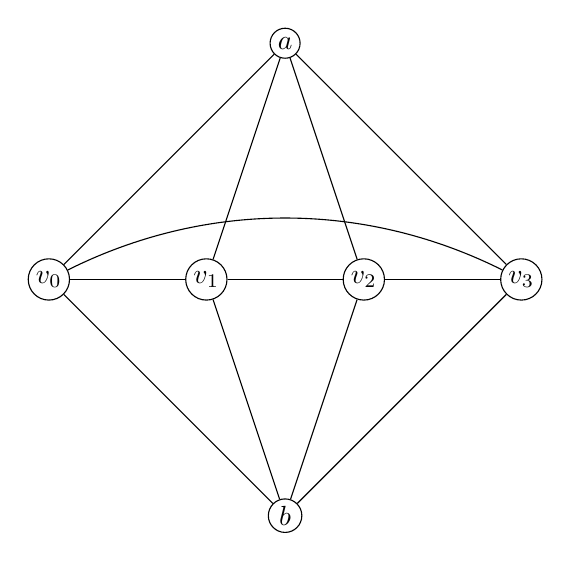
\begin{tikzpicture}[scale=1,every node/.style={draw,circle, inner sep=.05 cm}]
%top and bottom vertices placed by hand
\node (a) at (3,3){$a$};\node (b) at (3,-3){$b$}; 
%%middle vertices drawn with a loop
%% vertical edges drawn with a loop
\foreach \i in {0,1,2,3}{
	\node  (\i) at (2*\i,0){$v_{\i}$};
	\draw (a) -- (\i) -- (b);
	}
%% draw straight edges around the middle
\draw (0)--(1)--(2)--(3);
\draw (0) .. controls (2,1) and (4,1) .. (3);
\end{tikzpicture}
%%%END Graph G
&
%%%BEGIN Euler Tour
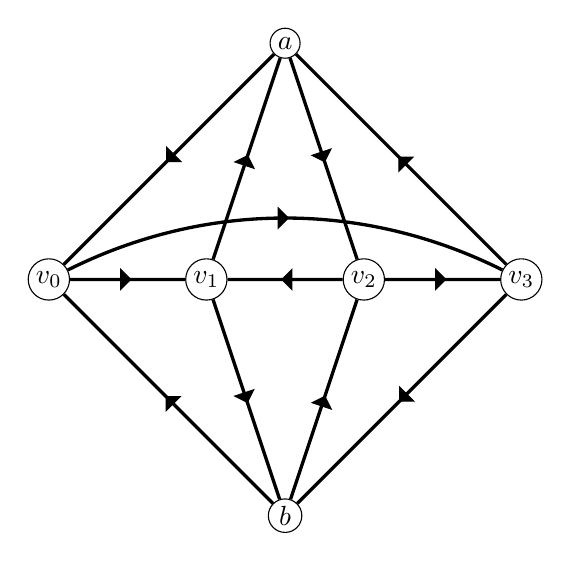
\begin{tikzpicture}[scale=1,every node/.style={draw,circle, inner sep=.05 cm}, every edge/.style = {draw, to reversed-to}]
%top and bottom vertices placed by hand
\node (a) at (3,3){$a$};\node (b) at (3,-3){$b$}; 
%%middle vertices drawn with a loop
\foreach \i in {0,1,2,3}{
	\node  (\i) at (2*\i,0){$v_{\i}$};
	}
%% draw euler tour
\begin{scope}[very thick, every node/.style={sloped,allow upside down}]
 \draw (a) -- node {\midarrow}(0)-- node {\midarrow} (1) -- node {\midarrow} (a) -- node {\midarrow}(2)-- node {\midarrow}(1)-- node {\midarrow}(b)-- node {\midarrow}(0) (3)-- node {\midarrow}(b)-- node {\midarrow}(2)-- node {\midarrow}(3)-- node {\midarrow}(a);
\draw (0)  .. controls (2,1) and (4,1) ..  node {\midarrow}(3);
\end{scope}
\end{tikzpicture}
%%%End Euler Tour
\end{tabular}
%%%End tablular environment
	\begin{enumerate}
	\item Find two nonisomorphic 2-factors in $G.$ Draw them using TikZ.
	\item Define a new graph $H$ with vertex set $V=\{a^+,a^-,b^+,b^-,v_0^+,v_0^-,v_1^+,v_1^-,v_2^+,v_2^-,v_3^+,v_3^-\}$ and edge set $E=\{ x^-y^+ \: \vert \: xy \in E(T) \text{ in that order }\}.$ Draw $H$ in TikZ.
	\item Explain why $H$ must (i) be bipartite and (i) satisfy Hall's condition.
	\item Find a 1-factor in $H$.
	\item Use the 1-factor in $H$ to find a 2-factor in $G.$ (For this problem it is sufficient to state the 1-factor and then state the 2-factor.)
	\end{enumerate}


\end{enumerate}
\end{document}


